% SC4013 --- Chapter 8: DevSecOps, Supply Chain, SBOM and Incident Response (0->100 ground-up)
\chapter{DevSecOps, Supply Chain, SBOM and Incident Response}
\label{ch:devsecops}

\begin{quote}
\emph{``You ship the dependency tree, not just your code.''} --- DevSecOps bakes security into the pipeline; supply-chain security proves what you shipped; incident response is the rehearsed playbook when prevention fails.
\end{quote}

\noindent\fbox{\parbox{\dimexpr\linewidth-2\fboxsep-2\fboxrule}{%
\textbf{From zero: how software is built and broken.} We assume no CI/CD or IR background. We walk from ``commit to deploy'' to ``SBOM to SLSA'' to ``detect to lessons learned,'' defining each term on first use.}}
\vspace{0.4em}

\section*{Learning Outcomes}
After this chapter you will be able to:
\begin{enumerate}[label=(L\arabic*)]
    \item place security gates in a CI/CD pipeline (shift left) and argue their order;
    \item explain supply-chain attacks (typosquat, hijack, build tamper) and mitigations;
    \item produce and consume an SBOM (SPDX/CycloneDX) and enforce it with SCA;
    \item describe SLSA levels and Sigstore signing for provenance;
    \item run the six-phase incident response lifecycle and write a post-mortem.
\end{enumerate}

% ============================================================
\section{DevSecOps: Shift Left in the Pipeline}
\label{sec:devsecops}
Intuition: fixing a bug in the IDE costs $1\times$, in code review $10\times$, in production $100\times$ (IBM/NIST). DevSecOps moves checks left --- closer to the commit --- so the cheapest fix wins.

\begin{figure}[h]\centering
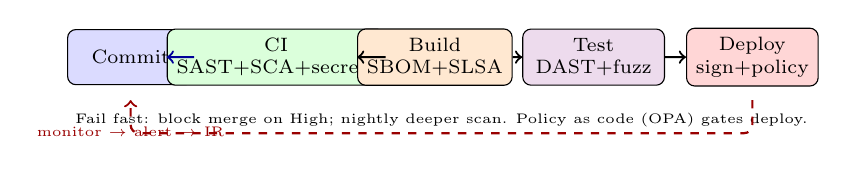
\begin{tikzpicture}[scale=0.84,every node/.style={font=\scriptsize}]
  \node[draw,fill=blue!14,rounded corners=3pt,minimum width=1.6cm,minimum height=0.7cm,align=center] (commit) at (-5.0,1.4) {Commit};
  \node[draw,fill=green!14,rounded corners=3pt,minimum width=1.8cm,minimum height=0.7cm,align=center] (ci) at (-2.8,1.4) {CI\\SAST+SCA+secrets};
  \node[draw,fill=orange!18,rounded corners=3pt,minimum width=1.8cm,minimum height=0.7cm,align=center] (build) at (-0.4,1.4) {Build\\SBOM+SLSA};
  \node[draw,fill=violet!14,rounded corners=3pt,minimum width=1.8cm,minimum height=0.7cm,align=center] (test) at (2.0,1.4) {Test\\DAST+fuzz};
  \node[draw,fill=red!16,rounded corners=3pt,minimum width=1.6cm,minimum height=0.7cm,align=center] (deploy) at (4.4,1.4) {Deploy\\sign+policy};
  \draw[->,thick,blue!60!black] (commit) -- (ci); \draw[->,thick] (ci) -- (build); \draw[->,thick] (build) -- (test); \draw[->,thick] (test) -- (deploy);
  \node[font=\tiny,align=center] at (-0.3,0.45) {Fail fast: block merge on High; nightly deeper scan. Policy as code (OPA) gates deploy.};
  \draw[->,thick,red!60!black,dashed,rounded corners=3pt] (4.4,0.75) -- (4.4,0.25) -- (-5.0,0.25) -- (-5.0,0.75) node[midway,below,font=\tiny] {monitor $\to$ alert $\to$ IR};
\end{tikzpicture}
\caption{DevSecOps pipeline. Each stage has a security gate; provenance (SLSA) and SBOM are produced at build and verified at deploy and in production.}
\label{fig:devsecops-pipe}
\end{figure}

Gates (in order): pre-commit (secrets, formatter), CI on every PR (SAST, SCA, secret scan, container scan with Trivy/Grype), build (generate SBOM, SLSA provenance, sign artifact with Sigstore), test (DAST/ZAP, fuzz with sanitizers), deploy (policy check: ``no Critical, no unreviewed dep''), and continuous (runtime guard, dependency update bot like Dependabot/Renovate). Keep gates fast ($<$5\,min for PR) or developers bypass them; run deep scans nightly.

Policy as code (OPA/Conftest, Sigstore Policy Controller) enforces ``image must be signed by CI, SLSA L3, no High CVE without waiver.'' Secrets never enter the repo: fetch from a vault at deploy, scan history with Gitleaks/TruffleHog.

% ============================================================
\section{Supply-Chain Security: Typosquat to Build Tamper}
\label{sec:supply-chain}
The SolarWinds, Codecov, Log4Shell and XZ incidents showed the same shape: the attacker did not breach \emph{your} code, they breached something your code trusts.

Attack classes:
\begin{description}[leftmargin=1.2em,itemsep=0.30em]
    \item[Typosquat / dependency confusion] \texttt{lodash} vs.\ \texttt{1odash}; private package name claimed on public registry.
    \item[Account hijack] Maintainer credential stolen; malicious version published.
    \item[Build tamper] CI compromised or build is irreproducible; artifact differs from source.
    \item[Transitive trust] You pin 10 deps; they pull 500 transitive deps. One is malicious.
\end{description}

\begin{figure}[h]\centering
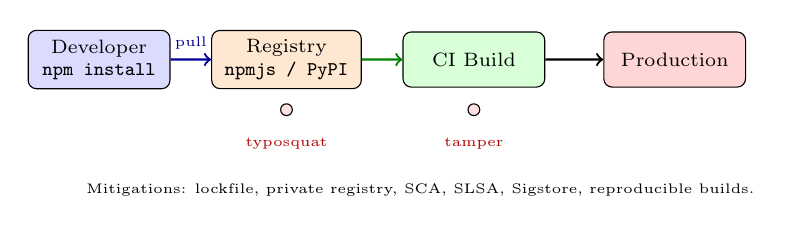
\begin{tikzpicture}[scale=0.85,every node/.style={font=\scriptsize}]
  \node[draw,fill=blue!14,rounded corners=3pt,minimum width=1.8cm,minimum height=0.7cm,align=center] (dev) at (-4.6,1.6) {Developer\\\texttt{npm install}};
  \node[draw,fill=orange!18,rounded corners=3pt,minimum width=1.9cm,minimum height=0.7cm,align=center] (reg) at (-1.8,1.6) {Registry\\\texttt{npmjs / PyPI}};
  \node[draw,fill=green!15,rounded corners=3pt,minimum width=1.8cm,minimum height=0.7cm,align=center] (ci) at (1.0,1.6) {CI Build};
  \node[draw,fill=red!16,rounded corners=3pt,minimum width=1.8cm,minimum height=0.7cm,align=center] (prod) at (4.0,1.6) {Production};
  \draw[->,thick,blue!60!black] (dev) -- (reg) node[midway,above,font=\tiny] {pull};
  \draw[->,thick,green!50!black] (reg) -- (ci);
  \draw[->,thick] (ci) -- (prod);
  \node[draw,fill=red!12,circle,inner sep=1.5pt] (x1) at (-1.8,0.85) {}; \node[font=\tiny,red!70!black] at (-1.8,0.35) {typosquat};
  \node[draw,fill=red!12,circle,inner sep=1.5pt] (x2) at (1.0,0.85) {}; \node[font=\tiny,red!70!black] at (1.0,0.35) {tamper};
  \node[font=\tiny,align=center] at (0.2,-0.35) {Mitigations: lockfile, private registry, SCA, SLSA, Sigstore, reproducible builds.};
\end{tikzpicture}
\caption{Supply-chain attack surface. Each arrow is a place where an attacker can inject code that you then ship as your own.}
\label{fig:supply-chain}
\end{figure}

Mitigations: lockfile + hash pinning, private registry proxy, SCA on every build, MFA + Sigstore for publishers, SLSA provenance, and reproducible builds that anyone can verify.

% ============================================================
\section{SBOM, SCA and SLSA/Sigstore}
\label{sec:sbom-slsa}
\begin{definition}[SBOM]
A \emph{Software Bill of Materials} is a machine-readable inventory of every component shipped: name, version, supplier, hash, license, and relationship. Standards: SPDX and CycloneDX (JSON/XML). Produced at build, stored with the artifact, checked at deploy.
\end{definition}

SCA (Dependabot, Snyk, Grype) matches the SBOM against CVE databases (OSV, NVD, GitHub Advisory) and flags vulnerable components. Gate: block deploy if a High is reachable (call graph) and unwaived.

\begin{lstlisting}[language=Python]
# Generate CycloneDX SBOM with cyclonedx-py, then scan with Grype
# pip install cyclonedx-bom
# cyclonedx-py -o sbom.json
# grype sbom:sbom.json -o json | jq '.matches[] | {name: .artifact.name, cve: .vulnerability.id}'
# Policy gate (Conftest/OPA): deny if any High without waiver
# data.deny[msg] { input.matches[_].vulnerability.severity == "High"; msg := "High CVE blocked" }
\end{lstlisting}

\begin{definition}[SLSA]
\emph{Supply-chain Levels for Software Artifacts} (SLSA, pronounced ``salsa'') levels 1--4 measure build integrity: L1 (provenance exists), L2 (hosted build, signed), L3 (hardened, non-falsifiable), L4 (hermetic, reproducible, two-party review).
\end{definition}

Sigstore (Fulcio + Rekor + Cosign) gives keyless signing: CI proves its identity via OIDC, gets an ephemeral cert, signs the artifact, and logs to a transparency ledger. Verification is \texttt{cosign verify --certificate-identity-regexp ...}. Together, SBOM says \emph{what} you ship, SLSA+Sigstore says \emph{where/how} it was built.

\begin{figure}[h]\centering
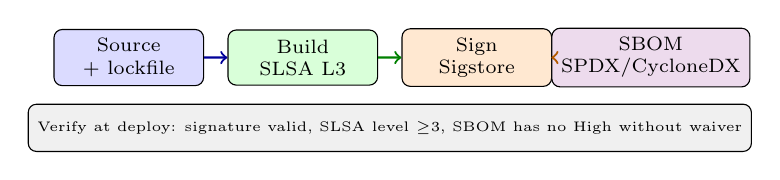
\begin{tikzpicture}[scale=0.85,every node/.style={font=\scriptsize}]
  \node[draw,fill=blue!14,rounded corners=3pt,minimum width=1.9cm,minimum height=0.7cm,align=center] (src) at (-3.8,1.4) {Source\\+ lockfile};
  \node[draw,fill=green!15,rounded corners=3pt,minimum width=1.9cm,minimum height=0.7cm,align=center] (build) at (-1.2,1.4) {Build\\SLSA L3};
  \node[draw,fill=orange!18,rounded corners=3pt,minimum width=1.9cm,minimum height=0.7cm,align=center] (sign) at (1.4,1.4) {Sign\\Sigstore};
  \node[draw,fill=violet!14,rounded corners=3pt,minimum width=1.9cm,minimum height=0.7cm,align=center] (sbom) at (4.0,1.4) {SBOM\\SPDX/CycloneDX};
  \draw[->,thick,blue!60!black] (src) -- (build); \draw[->,thick,green!50!black] (build) -- (sign); \draw[->,thick,orange!70!black] (sign) -- (sbom);
  \node[draw,fill=gray!12,rounded corners=3pt,minimum width=6.8cm,minimum height=0.6cm,align=center,font=\tiny] at (0.1,0.35) {Verify at deploy: signature valid, SLSA level $\ge$3, SBOM has no High without waiver};
\end{tikzpicture}
\caption{Provenance chain. Each artefact carries its SBOM and SLSA provenance; deploy verifies both before rollout.}
\label{fig:provenance}
\end{figure}

% ============================================================
\section{Incident Response and Post-Mortem}
\label{sec:ir}
No pipeline prevents all incidents. NIST SP 800-61 defines six phases: Prepare, Detect/Analyse, Contain, Eradicate, Recover, Lessons Learned. The goal is to shrink dwell time and prevent recurrence, not to assign blame.

\begin{description}[leftmargin=1.2em,itemsep=0.35em]
    \item[Prepare] Playbooks, logging, backups, and tabletop exercises (``secret leaked on GitHub,'' ``SBOM shows Log4Shell in prod''). If you have not rehearsed, you are not prepared.
    \item[Detect \& analyse] Alerts from monitoring/SCA/runtime; triage with CVSS + asset value; preserve evidence.
    \item[Contain] Short-term (revoke token, block IP, isolate host) then long-term (patch, firewall rule, feature flag).
    \item[Eradicate \& recover] Remove persistence, patch the root cause, restore from known-good, verify with tests/DAST.
    \item[Lessons learned] Blameless post-mortem, update pipeline/requirements so the bug class cannot return.
\end{description}

\begin{lstlisting}[language=Python]
# Minimal post-mortem template (store with the fix)
post_mortem = {
    "title": "Malicious transitive dep via typosquat lodahs@1.0.2",
    "severity": "High (CVSS 8.1) -- AV:N/AC:L/PR:N/UI:N/S:U/C:H/I:H/A:N",
    "root_cause": "No private registry proxy; CI pulled typosquat on clean cache",
    "fix": "Private registry + hash pin + SCA gate + SBOM diff in PR",
    "actions": ["registry proxy landed","SLSA L3 enforced","rekor verify in deploy"],
    "lessons": "Pipeline now fails closed on unknown package; IR tabletop added to onboarding"
}
\end{lstlisting}

Culture: blameless post-mortems, bias to fix the class not the instance, and mean-time-to-patch by severity as an engineering KPI. An incident that does not update the pipeline is a bug class waiting to fire again.

% ============================================================
\section{Containers, IaC and Runtime Guardrails}
\label{sec:containers-iac}
Containers and Infrastructure as Code (IaC) extend the supply chain. A Dockerfile like \texttt{FROM node:18} pulls 500\,MB including a shell, curl, and git---each a tool an attacker who gets RCE will use. Harden: use minimal base images (distroless, \texttt{alpine}), run as non-root (\texttt{USER 1001}), drop capabilities (\texttt{--cap-drop ALL}), and scan with Trivy/Grype in CI. IaC (Terraform, Helm, K8s YAML) is code: scan it with Checkov/KICS for misconfigurations (open S3 bucket, privileged pod, hostNetwork).

Runtime guardrails: admission controllers (OPA Gatekeeper, Kyverno) deny pods that are privileged or unsigned; runtime monitors (Falco, Tetragon) alert on anomalous syscalls (shell in a web container). Secrets in K8s \texttt{Secret} are base64, not encrypted by default---use Sealed Secrets or External Secrets with KMS.

\begin{example}[IaC misconfiguration]
Terraform \texttt{aws\_s3\_bucket: acl = "public-read"} is a breach waiting to happen. A Checkov rule flags it; the fix is \texttt{acl = "private"} + bucket policy + Block Public Access. Gate \texttt{terraform plan} in CI so no public bucket reaches prod, and drift detection alerts if someone changes it manually.
\end{example}

\begin{remark}[VEX and reachability]
A CVE without context is noise. VEX (Vulnerability Exploitability eXchange) lets the vendor state ``this CVE is not exploitable in your configuration.'' Combined with SBOM reachability, VEX suppresses false alarms so the team focuses on reachable Highs. Produce VEX alongside the SBOM and feed it to the SCA gate.
\end{remark}

\begin{remark}[Threat modeling in sprints]
DevSecOps is not a separate phase. In sprint planning, draw the DFD delta for the feature, STRIDE it (at least T/I/D on flows, S/E on processes), pick mitigations, and record residual risk as an ADR. The security champion in the team runs this in 30\,min; the artefact is a paragraph and a diagram, not a tome. No threat model, no merge for high-risk features.
\end{remark}

\begin{example}[Pipeline failure that caught a breach]
A PR added \texttt{left-pad 1.3.1} (typosquat). SCA flagged a High (malware), SBOM diff showed a new transitive dep, and the Conftest gate blocked merge. The developer had not noticed the typo. Without the gate, the package would have shipped to prod and exfiltrated \texttt{AWS\_SECRET\_ACCESS\_KEY} via install script---a real attack pattern seen on npm and PyPI.
\end{example}

\begin{remark}[Metrics that matter]
Track: (1)~time to fix by severity band, (2)~\% of features with a threat-model artefact, (3)~fuzz/DAST coverage trends, (4)~SAST true-positive rate, (5)~repeat-bug rate (same root cause twice). Review quarterly; a repeat bug means the last post-mortem did not land. Publish the dashboard; what gets measured gets fixed.
\end{remark}

\begin{remark}[Tabletop exercise]
Run a quarterly tabletop: ``SBOM shows Log4Shell in a vendor image that is already in prod.'' Walk Prepare through Lessons Learned with the actual people, tools and logs. Time how long to produce the list of affected services (SBOM query), to patch, and to verify. The slow step is where the pipeline needs investment.
\end{remark}

\begin{remark}[Audit readiness]
Auditors will ask for: SBOM for every release, SLSA provenance, SCA reports with disposition (fixed/waived with expiry), secret-scan logs, and IR tabletop records. Keep them as build artefacts in the registry, not as screenshots in a slide deck. An audit is a query over artefacts, not a story.
\end{remark}

\begin{example}[From IR to pipeline fix]
An incident where a leaked secret was in a GitHub fork led to the pipeline change: Gitleaks pre-commit hook + TruffleHog on every PR + secret revocation runbook + 1-hour SLA for High secrets. The post-mortem action was not ``remind developers'' but ``the push now fails closed.'' That is the class fix.
\end{example}

% ============================================================
\section{Exercises}
\label{sec:ch08-exercises}
\begin{enumerate}[label=E8.\arabic*, leftmargin=*, itemsep=0.6em]
    \item \textbf{Pipeline gates.} Map SAST, SCA, secret scan, SBOM generation, SLSA provenance, Sigstore signing, DAST and fuzzing to the commit$\to$deploy stages. Which gates block a PR in 5\,min vs.\ nightly? Justify ordering.
    \item \textbf{Supply-chain triage.} Your SCA flags Log4Shell (CVSS 10.0) in a transitive dep of a non-internet-facing batch job. Your API also has a Medium XSS on the payment page. Prioritise with CVSS + environmental metrics and state the next three commands/tickets for each.
    \item \textbf{SBOM diff.} A PR bumps \texttt{requests 2.28$\to$2.31}. Show the SBOM diff you expect, how Grype uses it, and the Conftest policy that blocks deploy if a High CVE without waiver is present.
    \item \textbf{Sigstore verify.} Sketch how \texttt{cosign sign} (Fulcio OIDC, ephemeral cert, Rekor ledger) and \texttt{cosign verify} work for a container image built on GitHub Actions. What does SLSA L3 add over L2 here?
    \item \textbf{IR tabletop.} A Sigstore verification fails at deploy: the image was built locally, not on CI. Walk the six IR phases, listing the first three actions in each of Contain, Eradicate and Lessons Learned, plus the post-mortem fields.
\end{enumerate}

\begin{remark}[Runtime drift]
A deployed container running with \texttt{--privileged} even though the image is signed and SBOM-clean shows why build-time checks are insufficient. Explain which runtime control (OPA Gatekeeper, seccomp, AppArmor) would block it and how to detect drift via continuous attestation.
\end{remark}

\begin{remark}[Provenance as policy]
Treat SLSA provenance as an admission controller input: only images with \texttt{builder.id == github-actions} and \texttt{source == main} at L3 are admitted to prod. This turns supply-chain metadata into a deploy-time policy, not just an audit artefact.
\end{remark}

\section*{Chapter Notes}
DevSecOps and shift-left are surveyed in Kim et al., \emph{The DevOps Handbook}, and NIST SSDF SP 800-218. Supply-chain attacks are catalogued in Ladisa et al.\ (2023) and SLSA (slsa.dev). SBOM standards are SPDX (ISO/IEC 5962) and CycloneDX (OWASP); OSV and NVD feed SCA. Sigstore is described at sigstore.dev; SLSA levels at slsa.dev/spec. Incident response follows NIST SP 800-61; blameless post-mortems from Allspaw and the SRE playbook.

% End of Chapter 8
